% ---------------------------------------------------------------------------
% The numbers of the "region" lines of string 1 (the -v log): how much of
% every light-cone piece each hadron ate. The + side has five pieces, the b
% and the four gluon halves; the - side the other four halves and the ubar.
% Every piece is drawn with unit length (they are not to scale: the b piece
% carries 165 GeV, the ubar piece 7). Red bites are hadrons from the b end,
% which eats the + side from the left and the - side from the left; blue
% bites are hadrons from the ubar end, which eats both from the right; grey
% is what was left for the final two. A hadron whose bites sit in more than
% one piece formed across a kink.
% ---------------------------------------------------------------------------
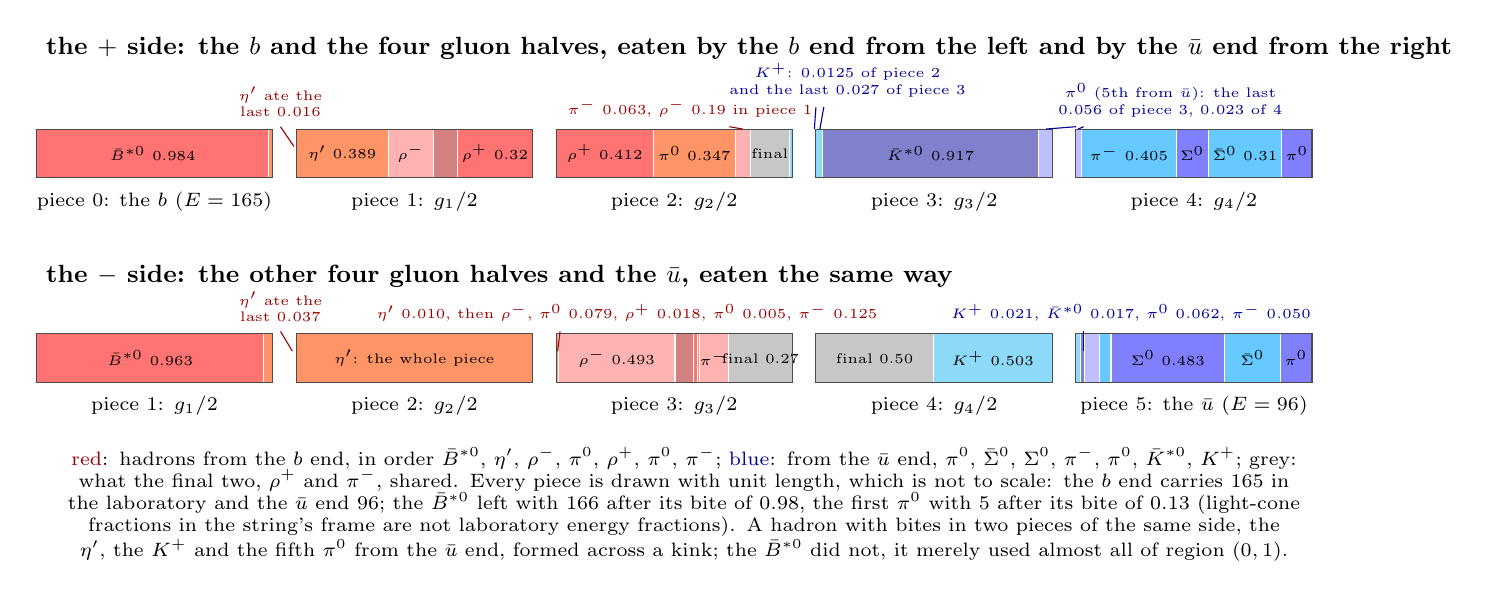
\begin{tikzpicture}[x=1cm,y=1cm,
  every node/.style={font=\footnotesize},
  lab/.style={font=\scriptsize,align=center},
  tiny/.style={font=\tiny,align=center},
  head/.style={font=\small\bfseries}]
% \pieceat{x0}{y}{list of frac/colour/label}: fills a 3 cm piece from the left
\def\pieceat#1#2#3{\xdef\px{#1}%
  \foreach \f/\c/\l in {#3} {%
    \pgfmathsetmacro{\w}{3*\f}%
    \fill[\c] (\px,#2) rectangle (\px+\w,#2+0.62);%
    \draw[white,line width=0.4pt] (\px,#2) -- (\px,#2+0.62);%
    \pgfmathsetmacro{\xm}{\px+\w/2}%
    \ifdim \w cm > 0.3cm \node[tiny] at (\xm,#2+0.31) {\l}; \fi%
    \pgfmathsetmacro{\nx}{\px+\w}\xdef\px{\nx}}%
  \draw[black!70] (#1,#2) rectangle (#1+3,#2+0.62);}
\colorlet{bA}{red!55!white}\colorlet{bB}{red!40!orange!60}\colorlet{bC}{red!30!white}\colorlet{bD}{red!65!black!50}
\colorlet{uA}{blue!50!white}\colorlet{uB}{blue!35!cyan!60}\colorlet{uC}{blue!25!white}\colorlet{uD}{blue!60!black!50}\colorlet{uE}{cyan!45!white}
\colorlet{fin}{black!22}
% ---------------- the + side -----------------------------------------------------------------------
\node[head,anchor=west] at (0,4.85) {the $+$ side: the $b$ and the four gluon halves, eaten by the $b$ end from the left and by the $\bar u$ end from the right};
\pieceat{0}{3.2}{0.9843/bA/{$\bar B^{*0}$ 0.984}, 0.0157/bB/{}}
\pieceat{3.3}{3.2}{0.3888/bB/{$\eta'$ 0.389}, 0.1919/bC/{$\rho^-$}, 0.1015/bD/{}, 0.3178/bA/{$\rho^+$ 0.32}}
\pieceat{6.6}{3.2}{0.4118/bA/{$\rho^+$ 0.412}, 0.3470/bB/{$\pi^0$ 0.347}, 0.0627/bC/{}, 0.1660/fin/{final}, 0.0125/uE/{}}
\pieceat{9.9}{3.2}{0.0265/uE/{}, 0.9171/uD/{$\bar K^{*0}$ 0.917}, 0.0564/uC/{}}
\pieceat{13.2}{3.2}{0.0228/uC/{}, 0.4048/uB/{$\pi^-$ 0.405}, 0.1328/uA/{$\Sigma^0$}, 0.3118/uB/{$\bar\Sigma^0$ 0.31}, 0.1278/uA/{$\pi^0$}}
\foreach \x/\t in {1.5/{piece 0: the $b$ ($E=165\GeV$)},4.8/{piece 1: $g_1/2$},8.1/{piece 2: $g_2/2$},11.4/{piece 3: $g_3/2$},14.7/{piece 4: $g_4/2$}} {\node[lab,anchor=north] at (\x,3.15) {\t};}
% leaders for the slivers on the + side
\node[tiny,anchor=south,text=red!60!black] at (3.1,3.85) {$\eta'$ ate the\\ last $0.016$};
\draw[thin,red!60!black] (3.1,3.85) -- (3.27,3.6);
\node[tiny,anchor=south,text=red!60!black] at (8.3,3.85) {$\pi^-$ $0.063$, $\rho^-$ $0.19$ in piece 1};
\draw[thin,red!60!black] (8.8,3.85) -- (8.97,3.82);
\node[tiny,anchor=south,text=blue!60!black] at (10.3,4.1) {$K^+$: $0.0125$ of piece 2\\ and the last $0.027$ of piece 3};
\draw[thin,blue!60!black] (9.9,4.1) -- (9.88,3.82); \draw[thin,blue!60!black] (10.0,4.1) -- (9.95,3.82);
\node[tiny,anchor=south,text=blue!60!black] at (14.4,3.85) {$\pi^0$ (5th from $\bar u$): the last\\ $0.056$ of piece 3, $0.023$ of 4};
\draw[thin,blue!60!black] (13.2,3.85) -- (12.82,3.82); \draw[thin,blue!60!black] (13.3,3.85) -- (13.23,3.82);
% ---------------- the - side -----------------------------------------------------------------------
\node[head,anchor=west] at (0,1.95) {the $-$ side: the other four gluon halves and the $\bar u$, eaten the same way};
\pieceat{0}{0.6}{0.9631/bA/{$\bar B^{*0}$ 0.963}, 0.0369/bB/{}}
\pieceat{3.3}{0.6}{1.0/bB/{$\eta'$: the whole piece}}
\pieceat{6.6}{0.6}{0.0103/bB/{}, 0.4932/bC/{$\rho^-$ 0.493}, 0.0786/bD/{}, 0.0183/bA/{}, 0.0051/bB/{}, 0.1245/bC/{$\pi^-$}, 0.27/fin/{final 0.27}}
\pieceat{9.9}{0.6}{0.4971/fin/{final 0.50}, 0.5029/uE/{$K^+$ 0.503}}
\pieceat{13.2}{0.6}{0.0206/uE/{}, 0.0165/uD/{}, 0.0622/uC/{}, 0.0496/uB/{}, 0.4825/uA/{$\Sigma^0$ 0.483}, 0.2344/uB/{$\bar\Sigma^0$}, 0.1342/uA/{$\pi^0$}}
\foreach \x/\t in {1.5/{piece 1: $g_1/2$},4.8/{piece 2: $g_2/2$},8.1/{piece 3: $g_3/2$},11.4/{piece 4: $g_4/2$},14.7/{piece 5: the $\bar u$ ($E=96\GeV$)}} {\node[lab,anchor=north] at (\x,0.55) {\t};}
\node[tiny,anchor=south,text=red!60!black] at (3.1,1.25) {$\eta'$ ate the\\ last $0.037$};
\draw[thin,red!60!black] (3.1,1.25) -- (3.25,1.0);
\node[tiny,anchor=south,text=red!60!black] at (7.5,1.25) {$\eta'$ $0.010$, then $\rho^-$, $\pi^0$ $0.079$, $\rho^+$ $0.018$, $\pi^0$ $0.005$, $\pi^-$ $0.125$};
\draw[thin,red!60!black] (6.65,1.25) -- (6.62,1.0);
\node[tiny,anchor=south,text=blue!60!black] at (13.9,1.25) {$K^+$ $0.021$, $\bar K^{*0}$ $0.017$, $\pi^0$ $0.062$, $\pi^-$ $0.050$};
\draw[thin,blue!60!black] (13.3,1.25) -- (13.3,1.0);
% ---------------- reading --------------------------------------------------------------------------
\node[lab,anchor=north west,text width=16.2cm] at (0,-0.1) {\textcolor{red!60!black}{red}: hadrons from the $b$ end, in order $\bar B^{*0}$, $\eta'$, $\rho^-$, $\pi^0$, $\rho^+$, $\pi^0$, $\pi^-$; \textcolor{blue!60!black}{blue}: from the $\bar u$ end, $\pi^0$, $\bar\Sigma^0$, $\Sigma^0$, $\pi^-$, $\pi^0$, $\bar K^{*0}$, $K^+$; grey: what the final two, $\rho^+$ and $\pi^-$, shared. Every piece is drawn with unit length, which is not to scale: the $b$ end carries $165\GeV$ in the laboratory and the $\bar u$ end $96\GeV$; the $\bar B^{*0}$ left with $166\GeV$ after its bite of $0.98$, the first $\pi^0$ with $5\GeV$ after its bite of $0.13$ (light-cone fractions in the string's frame are not laboratory energy fractions). A hadron with bites in two pieces of the same side, the $\eta'$, the $K^+$ and the fifth $\pi^0$ from the $\bar u$ end, formed across a kink; the $\bar B^{*0}$ did not, it merely used almost all of region $(0,1)$.};
\end{tikzpicture}
